\documentclass{standalone}
\usepackage{tikz}
\usetikzlibrary{positioning, circuits.ee.IEC, decorations.pathreplacing}

\begin{document}
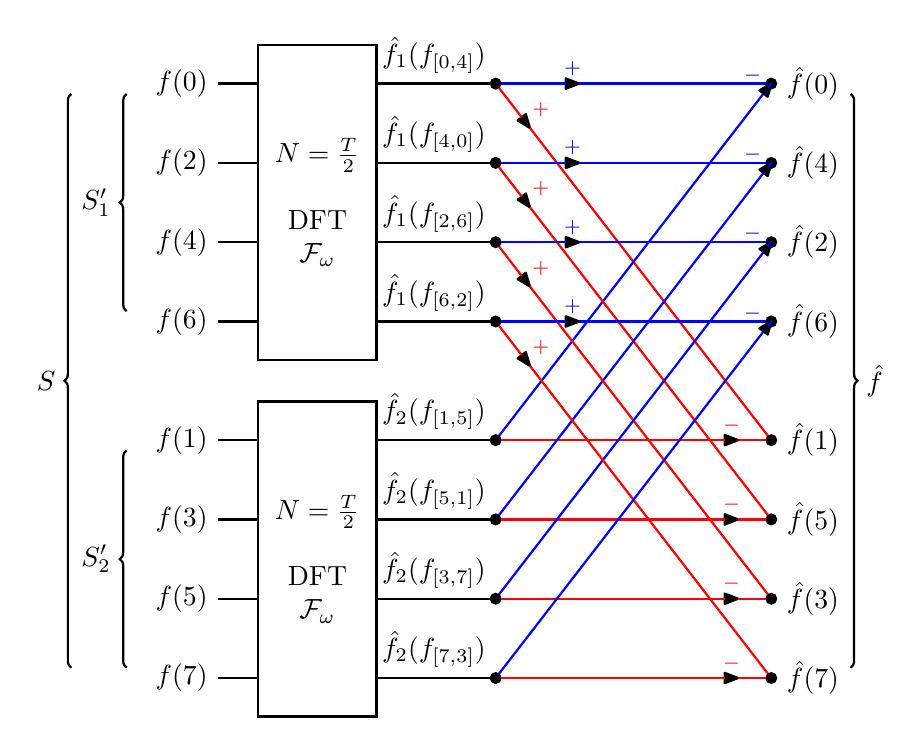
\begin{tikzpicture}
% Style
[
    thick, node distance=.5cm, circuit ee IEC,
    box/.style={
        draw, align=center, shape=rectangle, minimum width=1.5cm, minimum height=4cm,
        append after command={% see also: https://tex.stackexchange.com/a/129668
            \foreach \side in {east,west} {
                \foreach \i in {1,...,#1} {
                %  oordinate (\tikzlastnode-\i-\side)
                %  at ($(\tikzlastnode.north \side)!{(\i-.5)/(#1)}!(\tikzlastnode.south \side)$)
                    (\tikzlastnode.north \side) edge[draw=none, line to]
                        coordinate[pos=(\i-.5)/(#1)] (\tikzlastnode-\i-\side) (\tikzlastnode.south \side)
                }
            }
        }
    }
]

%=================================== Start ===================================
{
    \node[box=4] (box-t) {$N = \frac{T}{2}$ \\\\ DFT \\ ${\mathcal {F}}_{\omega}$};
    \node[box=4, below=of box-t] (box-b) {$N = \frac{T}{2}$ \\\\ DFT \\ ${\mathcal {F}}_{\omega}$};

    \foreach \s[count=\i] [
        evaluate={\sa=int(\s*2)},
        evaluate={\sb=int(\s*2+1)}
    ] in {0,1,2,3} {
        \path (box-t-\i-west) edge node[at end, left](f-t-\i){$f({\sa})$} ++(left:.5);
        \path (box-b-\i-west) edge node[at end, left](f-b-\i){$f({\sb})$} ++(left:.5);
    }
    \foreach \b/\s[count=\k] in {t/1} {
        \foreach \i /\r /\a /\j in {1/1/f_{[0,4]}/0, 2/1/f_{[4,0]}/4, 3/1/f_{[2,6]}/2,4/1/f_{[6,2]}/6} {
            \node [contact] (conn-\b-\i) at ([shift=(right:1.5)] box-\b-\i-east) {}
            edge node[above] {$\hat{f}_{\r}(\a)$} (box-\b-\i-east)
            node [contact, label=right:{$\hat{f}(\j)$}](conn-\b-\i') at ([shift=(right:5)] box-\b-\i-east) {};
        }
    }  
    \foreach \b/\s[count=\k] in {b/2} {
        \foreach \i /\r /\a /\J in {1/2/f_{[1,5]}/1,2/2/f_{[5,1]}/5,3/2/f_{[3,7]}/3,4/2/f_{[7,3]}/7} {
            \node [contact] (conn-\b-\i) at ([shift=(right:1.5)] box-\b-\i-east) {}
            edge node[above] {$\hat{f}_{\r}(\a)$} (box-\b-\i-east)
            node [contact, label=right:{$\hat{f}(\J)$}](conn-\b-\i') at ([shift=(right:5)] box-\b-\i-east) {};
        }
    }  

    \node (S-1-0) [left=of f-t-1, left=3pt] {};
    \node (S-1-1) [left=of f-t-4, left=3pt] {};
    \node (S-2-0) [left=of f-b-1, left=3pt] {};
    \node (S-2-1) [left=of f-b-4, left=3pt] {};
    \node (S-1) [left=of f-t-1, left=23pt] {};
    \node (S-2) [left=of f-b-4, left=23pt] {};
    \draw[decorate, decoration={brace,mirror}] (S-1-0) -- node[left=2pt] {$S^{\prime}_1$} (S-1-1);
    \draw[decorate, decoration={brace,mirror}] (S-2-0) -- node[left=2pt] {$S^{\prime}_2$} (S-2-1);
    \draw[decorate, decoration={brace,mirror}] (S-1) -- node[left=2pt] {$S$} (S-2);

    \node (O-1) [right=of conn-t-1', right=23pt] {};
    \node (O-2) [right=of conn-b-4', right=23pt] {};
    \draw[decorate, decoration={brace}] (O-1) -- node[right=2pt] {$\hat{f}$} (O-2);

    \begin{scope}[every info/.append style={font=\scriptsize, inner sep=+.5pt}]
    {
        \foreach \i [
            evaluate={\j=int(\i-1)},
            evaluate={\J=int(\i+3)}
        ] in {1,...,4} {
            \path (conn-t-\i) edge[current direction={pos=.27 , info=$+$           },blue] (conn-t-\i');
            \path (conn-t-\i) edge[current direction={pos=.1  , info=$+$           },red ] (conn-b-\i');
            \path (conn-b-\i) edge[current direction={pos=.87 , info={$-$}},red ] (conn-b-\i');
            \path (conn-b-\i) edge[current direction={pos=.999, info={$-$}},blue] (conn-t-\i');
        }
    }
    \end{scope}
}
%==================================== END ====================================

\end{tikzpicture}
\end{document}